\documentclass[introducao.tex]{subfiles}
\begin{document}
\section{Introdução}
\paragraph{} A equação de Navier Stokes é apresentada abaixo, essa é a equação que governa a dinâmica dos fluidos.

\begin{eqnarray}
\rho\left( \frac{\partial {\textbf{v}}}{\partial t}+\textbf{v}\cdot\nabla \textbf{v} \right)=-\nabla p+\mu\nabla^2 \textbf{v} + \textbf{f}\label{navierstokes}\\
\nabla\cdot\textbf{v}=0
\end{eqnarray}

\paragraph{} Neste trabalho consideraremos um campo vetorial de duas dimensões. A equação de Navier Stokes é fortemente não-linear. Isso ocorre devido aos termos de convecção (aceleração independente do tempo, $\textbf{v}\cdot \nabla\textbf{v}$) e gradiente de pressão ($\nabla p$). 

\paragraph{} A abordagem para se obter uma solução para a equação dos fluidos é de seguir o método de Chorin\cite{chorin68} com malha escalonada. Para cada passo de tempo, há 3 etapas a serem realizadas. Será utilizado \textit{time-splitting} de forma a se desacoplar a pressão da velocidade, ambas incógnitas. 

\paragraph{} O que deve ser definido antes de se resolver tal equação são os parâmetros do fluido, $\mu$ e $\rho$ (massa específica), a força externa $\textbf{f}$ e as condições de fronteira. Nosso interesse inicial é resolver o problema da cavidade num quadradro de lado igual a 1 numa malha de $n$ pontos. As condições de fronteira são $u(x,1)=\sin{\pi x}^2$ e zero caso contrário.
\paragraph{} A seguir será feita uma introdução do que vem a ser \textit{time-splitting}, de forma a se compreender este trabalho.

\subsection{Time-splitting} A primeira etapa neste método de resolução é o \textit{time-splitting}. A discretização no tempo tem duas etapas. Para se entender isso, começamos com a equação abaixo:
\begin{equation}
\frac{\partial \textbf{v}}{\partial t}\approx \frac{\textbf{v}^{n+1}-\textbf{v}^n}{\Delta t}=\frac{\textbf{v}^{n+1}-\textbf{v}^*}{\Delta t}+\frac{\textbf{v}^{*}-\textbf{v}^n}{\Delta t} 
\end{equation}

\paragraph{} A ideia do \textit{time-splitting} é responsabilizar cada um dos termos do lado direito desta equação com uma parte da equação de Navier-Stokes. Reescrevendo a equação de Navier-Stokes:

\begin{eqnarray*}
\frac{\textbf{v}^{n+1}-\textbf{v}^*}{\Delta t}+\frac{\textbf{v}^{*}-\textbf{v}^n}{\Delta t}=-\frac{1}{\rho}\nabla p + \nu\nabla ^2 \textbf{v} + \frac{\textbf{f}}{\rho} - \textbf{v}\cdot \nabla \textbf{v}
\end{eqnarray*}

Agora, é possível impor o seguinte:

\begin{eqnarray}
\frac{\textbf{v}^{*}-\textbf{v}^n}{\Delta t}&=& \nu\nabla ^2 \textbf{v} + \frac{\textbf{f}}{\rho} - \textbf{v}\cdot \nabla \textbf{v}\label{equacaovestrela}\\
\frac{\textbf{v}^{n+1}-\textbf{v}^*}{\Delta t}&=&-\frac{1}{\rho}\nabla p\label{equacaoprepressao}
\end{eqnarray}

A equação \ref{equacaovestrela} pode ser discretizada e então obtemos $\textbf{v}^*$. A equação \ref{equacaoprepressao}, por sua vez, não pode ser diretamente discretizada e resolvida pois não se sabe $\textbf{v}^{n+1}$. No entanto, se o gradiente da equação for obtido, tem-se:

\begin{eqnarray*}
\nabla\cdot \left(\frac{\textbf{v}^{n+1}-\textbf{v}^*}{\Delta t}\right)&=&\nabla\cdot\frac{\textbf{v}^{n+1}}{\Delta t}-\nabla\cdot \frac{\textbf{v}^*}{\Delta t}\\
&=&-\frac{1}{\rho}\nabla^2 p
\end{eqnarray*}

A equação da continuidade $\nabla\cdot \textbf{v}=0$ tem de valer para $\textbf{v}^{n+1}$, logo:

\begin{eqnarray}
\nabla^2 p = \frac{\rho}{\Delta t}\nabla\cdot\textbf{v}^*\label{eqpressao}
\end{eqnarray}

Nos próximos passos, iremos fazer o seguinte:

\begin{enumerate}
\item obter $\textbf{v}^*$, que seria o intermediário entre $\textbf{v}^n$ e $\textbf{v}^{n+1}$
\item  obter a pressão, $p$
\item obter $\textbf{v}^{n+1}$
\end{enumerate}

\subsection{Malha escalonada}
\paragraph{} De forma sintética: o uso de uma malha normal pode gerar modos espúrios de pressão indesejados. Uma outra forma de representar os dados nas matrizes é a escalonada. Nela, o ponto $ij$, ao invés de representar a velocidade $\textbf{v}(i\Delta x, j\Delta y)$, representará a velocidade  $u(i\Delta x, (j+\frac{1}{2})\Delta x)$ e $v((i+\frac{1}{2})\Delta x, j\Delta x)$. Logo, ao invés de um ponto $ij$ é melhor pensar num pequeno quadrado de índice $ij$ que contém as velocidades, pressão e força utilizadas em nosso problema. Consideramos a força em $x$ e $y$ na mesma posição que as velocidades. A pressão permanece no centro do quadrado. A figura abaixo ilustra isso:

\begin{center}
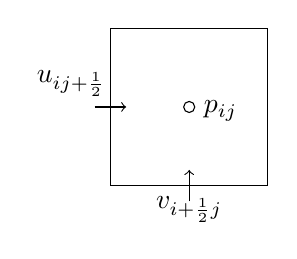
\begin{tikzpicture}
\draw (0,0) rectangle (2,2);
\draw (1.4,0.95) node {$p_{ij}$};
\draw[->] (1,-0.2) -- (1,0.2);
\draw (1,-0.3) node {$v_{i+\frac{1}{2}j}$};
\draw[->] (-0.2,1) -- (0.2,1);
\draw (-0.5,1.3) node {$u_{ij+\frac{1}{2}}$};
\draw (1,1) circle (2pt);
\end{tikzpicture}
\end{center}

\paragraph{} Uma representação de um domínio mais completo está na figura abaixo. Note que cada ponto preto no meio de um bloco é a pressão em ponto interno. Enquanto a pressão em pontos da fronteira imaginária são círculos com interior branco. Pontos na fronteira imaginária são utilizados nos cálculos, mas não precisam ser salvos no resultado final.

\paragraph{} Se é definida, no computador, uma matriz $n\times n$, tem-se $\Delta x = \frac{1}{n-2}$. Os cálculos devem ser todos feitos com base neste $\Delta x$. Além disso, note que as velocidades da extrema esquerda e do extremo inferior não são utilizadas. Você pode declarar tais valores como Not a Number. Se seu programa utilizá-los, há algo errado.

\domainOne

\subsection{Diferenças finitas não-simétricas}

\paragraph{} Em virtude de um erro maior do que o esperado, apesar de decair com o quadrado de $\Delta x$, as fronteiras do problema de Poisson com condições de Neumann necessitam de diferenças finitas de quarta ordem. Para isso, considere a figura abaixo:

\nonsymmetricright
%\nonsymmetricleft

\paragraph{} Os pontos vermelhos serão utilizados. O que se deseja é a derivada no ponto $p_{0.5} = p(0.5)$, isto é:

\begin{eqnarray}
\left.\frac{\partial p}{\partial x}\right|_{0.5} & = & a_0 p_0 + a_{0.5} p_{0.5} + a_1 p_1 + a_2 p_2 + a_3 p_3\label{combinationNonSymmetric}
\end{eqnarray}

\paragraph{} Para isso, desenvolvemos os valores de $p_i$ por meio de série de Taylor. Assim:

\begin{eqnarray}
p_0 & = & p(0.5) - \frac{\Delta x}{2}p'(0.5) + \frac{\Delta x^2}{4}p''(0.5) - \frac{\Delta x^3}{8} p^{(3)}(0.5) + \frac{\Delta x^4}{16} p^{(4)}(0.5) \nonumber\\
p_{0.5} & = & p(0.5) \nonumber \\
p_1 & = & p(0.5) + \frac{\Delta x}{2}p'(0.5) + \frac{\Delta x^2}{4}p''(0.5) + \frac{\Delta x^3}{8} p^{(3)}(0.5) + \frac{\Delta x^4}{16} p^{(4)}(0.5)\nonumber \\
p_2 & = & p(0.5) + \left(\frac{3\Delta x}{2}\right)p'(0.5) + \left(\frac{9\Delta x^2}{4}\right)p''(0.5) + \left(\frac{27\Delta x^3}{8}\right)p^{(3)}(0.5)+\left(\frac{81\Delta x^4}{16}\right)p^{(4)}(0.5)\nonumber\\
p_3 & = & p(0.5) + \left(\frac{5\Delta x}{2}\right)p'(0.5) + \left(\frac{25\Delta x^2}{4}\right)p''(0.5) + \left(\frac{125\Delta x^3}{8}\right)p^{(3)}(0.5)+\left(\frac{625\Delta x^4}{16}\right)p^{(4)}(0.5)\nonumber
\end{eqnarray}
 
\paragraph{} Trocando $p_i$ na equação \ref{combinationNonSymmetric} pelas suas representações com série de Taylor, tem-se um sistema linear para obter as constantes $a_i$.

\begin{eqnarray}
\left[\begin{array}{ccccc}
1 & 1 & 1 & 1 & 1\\
-\frac{\Delta x}{2} & 0 & \frac{\Delta x}{2} & \frac{3\Delta x}{2} & \frac{5\Delta x}{2}\\
\frac{\Delta x^2}{4} & 0 & \frac{\Delta x^2}{4} & \frac{9\Delta x^2}{4} & \frac{25\Delta x^2}{4}\\
-\frac{\Delta x^3}{8} & 0 & \frac{\Delta x^3}{8} & \frac{27\Delta x^3}{8} & \frac{125\Delta x^3}{8}\\
\frac{\Delta x^4}{16} & 0 & \frac{\Delta x^4}{16} & \frac{81\Delta x^4}{16} & \frac{625\Delta x^4}{16}\\
\end{array}\right]\left[\begin{array}{c}a_0\\ a_{0.5}\\ a_1\\ a_2\\ a_3\end{array}\right] & = & \left[\begin{array}{c}0\\ 1\\ 0\\ 0\\ 0\end{array}\right]
\end{eqnarray}

\paragraph{} Assim que são obtidos os valores dos coeficientes $a_i$, iremos isolar $p_0$:

\begin{eqnarray}
p_0 & = & \frac{1}{a_0}\left(a_{0.5}p_{0.5} + a_1 p_1 + a_2 p_2 + a_3 p_3 - \left.\frac{\partial p}{\partial x}\right|_{0.5}\right)
\end{eqnarray}

\paragraph{} Desenvolvimento similar deve ser feito para o outro lado:

\nonsymmetricleft

\paragraph{} Assim:

\begin{eqnarray}
p_n & = & p_{n-0.5} + \frac{\Delta x}{2}p'_{n-0.5} + \frac{\Delta x^2}{4}p''_{n-0.5} + \frac{\Delta x^3}{8} p^{(3)}_{n-0.5} + \frac{\Delta x^4}{16} p^{(4)}_{n-0.5} \nonumber\\
p_{n-0.5} & = & p_{n-0.5} \nonumber \\
p_{n-1} & = & p_{n-0.5} - \frac{\Delta x}{2}p'_{n-0.5} + \frac{\Delta x^2}{4}p''_{n-0.5} - \frac{\Delta x^3}{8} p^{(3)}_{n-0.5} + \frac{\Delta x^4}{16} p^{(4)}_{n-0.5}\nonumber \\
p_{n-2} & = & p_{n-0.5} - \left(\frac{3\Delta x}{2}\right)p'_{n-0.5} + \left(\frac{9\Delta x^2}{4}\right)p''_{n-0.5} - \left(\frac{27\Delta x^3}{8}\right)p^{(3)}_{n-0.5}+\left(\frac{81\Delta x^4}{16}\right)p^{(4)}_{n-0.5}\nonumber\\
p_3 & = & p_{n-0.5} - \left(\frac{5\Delta x}{2}\right)p'_{n-0.5} + \left(\frac{25\Delta x^2}{4}\right)p''_{n-0.5} - \left(\frac{125\Delta x^3}{8}\right)p^{(3)}_{n-0.5}+\left(\frac{625\Delta x^4}{16}\right)p^{(4)}_{n-0.5}\nonumber
\end{eqnarray}

\paragraph{} E temos:

\begin{eqnarray}
\left[\begin{array}{ccccc}
1 & 1 & 1 & 1 & 1\\
\frac{\Delta x}{2} & 0 & -\frac{\Delta x}{2} & -\frac{3\Delta x}{2} & -\frac{5\Delta x}{2}\\
\frac{\Delta x^2}{4} & 0 & \frac{\Delta x^2}{4} & \frac{9\Delta x^2}{4} & \frac{25\Delta x^2}{4}\\
\frac{\Delta x^3}{8} & 0 & -\frac{\Delta x^3}{8} & -\frac{27\Delta x^3}{8} & -\frac{125\Delta x^3}{8}\\
\frac{\Delta x^4}{16} & 0 & \frac{\Delta x^4}{16} & \frac{81\Delta x^4}{16} & \frac{625\Delta x^4}{16}\\
\end{array}\right]\left[\begin{array}{c}b_0\\ b_{0.5}\\ b_1\\ b_2\\ b_3\end{array}\right] & = & \left[\begin{array}{c}0\\ 1\\ 0\\ 0\\ 0\end{array}\right]
\end{eqnarray}

\paragraph{} Uma vez obtidos os coeficientes:

\begin{eqnarray}
\left.\frac{\partial p}{\partial x}\right|_{n-0.5} & = & b_0 p_n + b_{0.5} p_{n-0.5} + b_1 p_{n-1} + b_2 p_{n-2} + b_3 p_{n-3}\\
p_n & = & \frac{1}{b_0}\left(b_{0.5} p_{n-0.5} + b_1 p_{n-1} + b_2 p_{n-2} + b_3 p_{n-3} - \left.\frac{\partial p}{\partial x}\right|_{n-0.5}\right)
\end{eqnarray}



\end{document}
